%!TEX root = ../main.tex
\section{Assessing pipelines configured from \isklearn}
\label{sec:results}

To evaluate our proposal, we take ensembles produced by \autosklearn as baseline. As discussed, the focus of our investigation is on computer vision~(CV), natural language processing~(NLP), and time series~(TS) prediction problems. The Auto-WEKA and \autosklearn works used tabular and CV datasets as benchmarks. Among the CV ones, the most relevant are 
% specifically the ones However, for this first assessment of \isklearn, we filtered out small datasets~(less than 10\,000 samples) and datasets that~(i)~presented significant class balancing issues; (ii)~comprised mostly categorical features, and/or; (iii)~were variants of better-known datasets. Unfortunately, out of the 21 datasets originally considered in~\cite{auto-sklearn}, only the 
the MNIST and CIFAR-10 classification datasets. However, since the differences in performance between algorithms is generally rather small for MNIST, we replace it with the more challenging Fashion MNIST~(FMNIST). We additionally consider SVHN, a house number recognition problem. Regarding the remaining application domains, we included: (i)~three NLP classification datasets, namely LMRD for sentiment analysis, and Reuters and AGNews for topic classification, and; (ii)~two TS analysis regression datasets, concerning crime incidence prediction~\cite{kounadi2020systematic} in the cities of Boston, MA, EUA, and Natal, RN, Brazil. Further information on these datasets is given in the supplementary material, particularly the details on manual data preparation, sampling, and resource limits for \autosklearn.


% \begin{table*}[]
% \centering
% \caption{\small iSklearn-configured pipeline overview for each dataset}
% \label{tb:pipelines}
% \scalebox{0.8}{
% \begin{tabular}{*{8}{l}}
% \hline
% & & \textbf{MNIST} & \textbf{CIFAR-10} & \textbf{LMRD} & \textbf{Reuters} & \textbf{Natal} & \textbf{Boston} \\ \hline
% \multirow{4}{*}{\texttt{Preprocessing}} 	& \texttt{Scaling} & True & False & False  & False & True & False \\ \cline{2-8}
% & \multirow{2}{*}{\texttt{FE}$_1$} & \texttt{Selection} & \multirow{2}{*}{---} & \texttt{Selection}  & \texttt{Selection}  & \texttt{Selection} & \texttt{Selection} \\
% & & (\emph{model}: RF) & & (\emph{model}: RF)  & (\emph{model-free})  & (\emph{model}: SVM) & (\emph{model}: SVM) \\ \cline{2-8}
% & \multirow{2}{*}{\texttt{FE}$_2$} & \multirow{2}{*}{---} & \multirow{2}{*}{---} & \multirow{2}{*}{---}  & \texttt{Extraction}  & \multirow{2}{*}{---} & \texttt{Extraction} \\
% 	&  &  &  &   & (SVD) & & (ICA) \\ \hline
% \multirow{2}{*}{\texttt{Prediction}} 	& \texttt{Scaling} & True & True & False  & False  & False & False \\ \cline{2-8}
% 								& \texttt{Predictor} & SVM & kNN & SVM  & MLP  & LR & LR \\ \hline
% \end{tabular}}
% \end{table*}

%\newpage

Since \irace and SMAC are heuristic algorithms, we report results from 10 runs of both \isklearn and \autosklearn on each dataset.
A single run of \isklearn on a given dataset has a configuration budget of $2\,000$ experiments. An experiment is defined as evaluating a candidate configuration on a given instance~(tuple of $p$ meta-folds). In the assessment done in this section, we set $p=1$ to isolate the effect of changing the bottom-level sampling; alternative $p$ values will be assessed in Section~\ref{sec:alt-setups}. Maximum runtime for each experiment is set to 10 minutes. If the evaluation of a configuration exceeds this limit, the configuration is penalized so that \irace may discard it at the end of the iteration. After pipelines are configured from \isklearn, we validate them on the test samples and report mean performance and variance over the 10 runs. Following the literature, both configuration and validation are guided by accuracy for classification tasks and $R^2$ for regression tasks. 
%Furthermore, since \irace and SMAC are heuristic algorithms, we report results from 10 runs of both \isklearn and \autosklearn.

We start by analyzing pipeline structures selected by \irace for each applicaton domain, given as sunburst plots in Figure~\ref{fig:domain_composition}. FE$_1$ and FE$_2$ depict the possibility of using \texttt{\small Selection} and \texttt{\small Extraction} simultaneously -- if only one of them is used, it is depicted as FE$_1$. 
%When either \texttt{\small Selection} or \texttt{\small Extraction} is adopted, its associated strategy is reported in parenthesis. 
The two most important insights we observe are the differences in composition between domains and also datasets. 
In order, composition for NLP, CV, and TS use increasingly more preprocessing components. While pipelines from all domains use \texttt{\small Extraction} a few times, TS pipelines additionally always use \texttt{\small Selection}. Use of different prediction options increases in a different order, with NLP being the domain where the least different alternatives are chosen, and CV the one where the most are. Regarding NLP, 29 out of the 30 pipelines devised adopt LR. This algorithm is also most frequently chosen for TS datasets, followed by SVM and MLP. Finally, we notice that more complex predictors such as ensemble methods are only once selected~(AB for SVHN).

We further assess pipeline composition as a function of the given dataset. For brevity, sunburst plots for each dataset are provided as supplementary material. First, a different predictor is mostly selected for each of the CV problems, namely LR for CIFAR-10, SVM for FMNIST, and kNN for SVHN. In addition, preprocessing is increasingly adopted in these datasets, in this order. Concerning TS problems, LR is frequently selected for the Boston dataset, followed by SVM, whereas for the Natal dataset SVM, LR, and MLP are uniformly distributed. Preprocessing patterns for TS problems are little affected by the particularities of each dataset. Finally, in NLP, preprocessing is only adopted more than once for Reuters, mostly through \texttt{\small Extraction}.
% For instance, lack of clear-cut patterns, which reinforces the need for AutoML approaches. Yet, we do observe common practices from experienced ML designers, with different estimators employed for selection and prediction in a same pipeline. We also remark how much more often component \texttt{\small Selection} is adopted in contrast to \texttt{\small Extraction}.   

\begin{figure*}
    \centering
    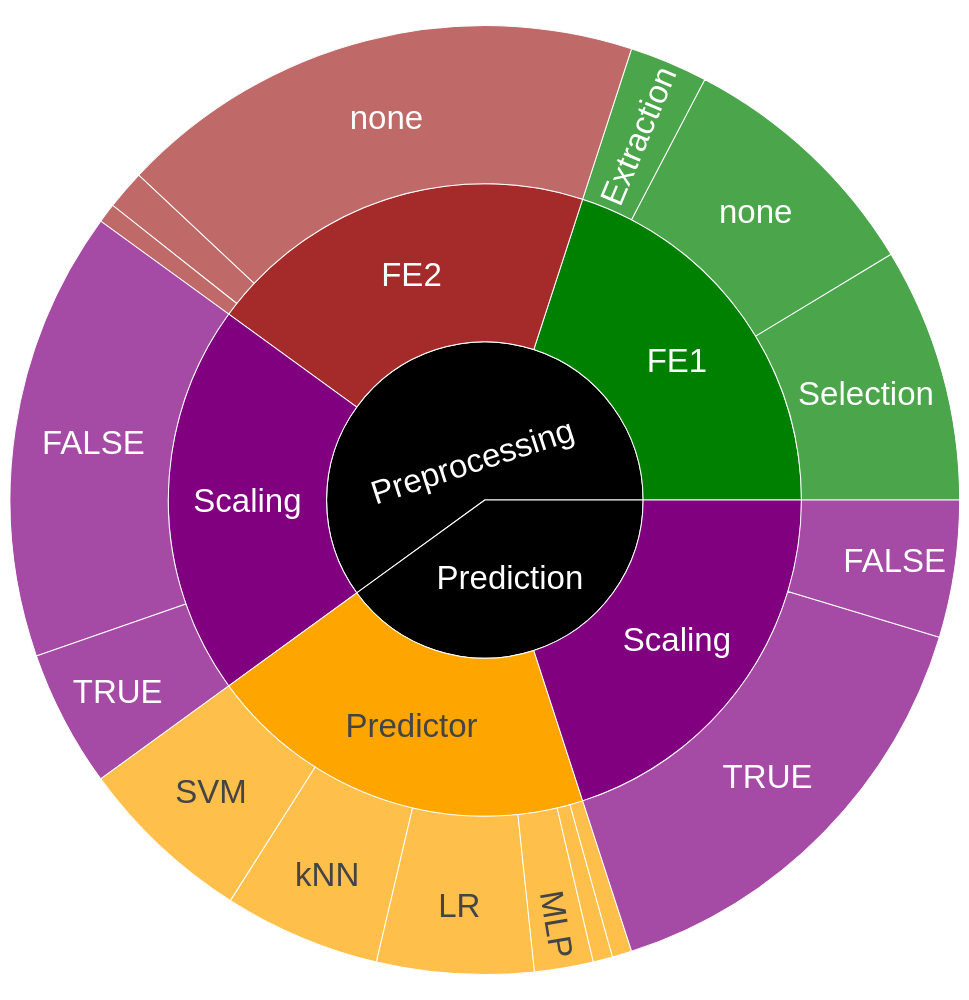
\includegraphics[width=5.5cm]{img/sunburst/cv.png}
    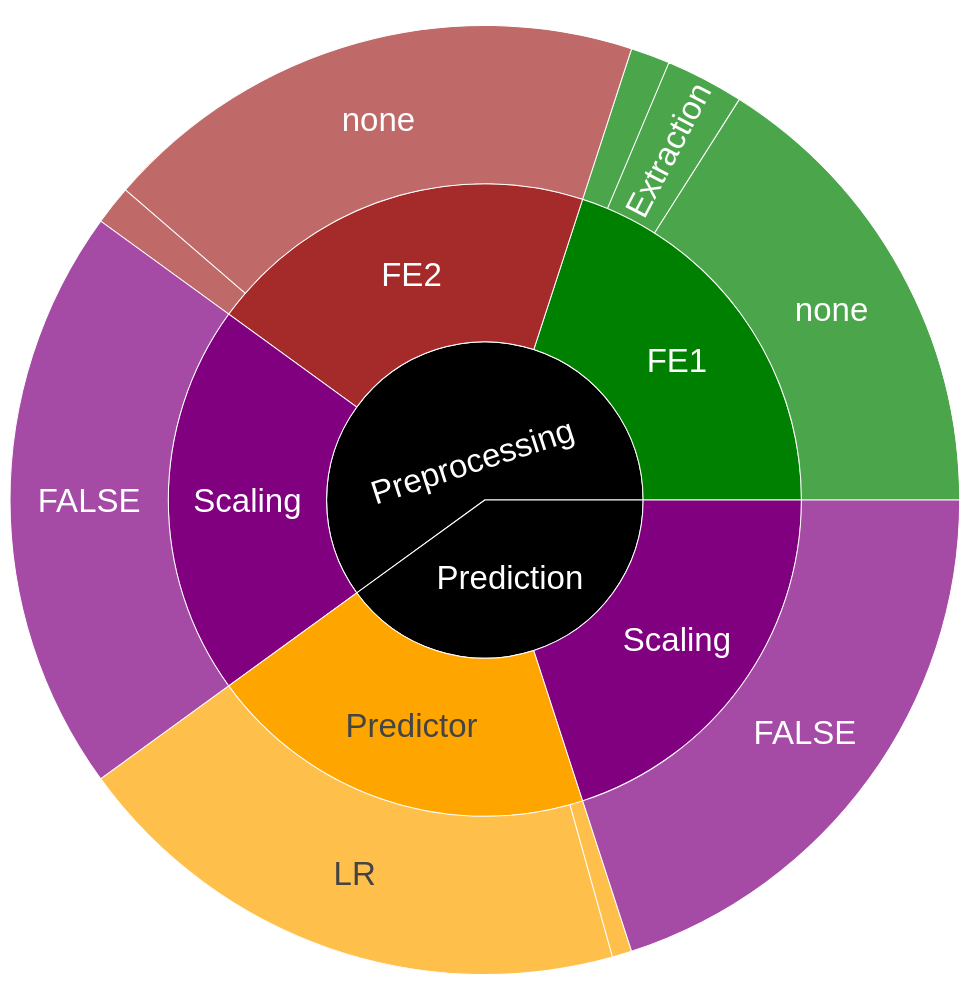
\includegraphics[width=5.5cm]{img/sunburst/nlp.png}
    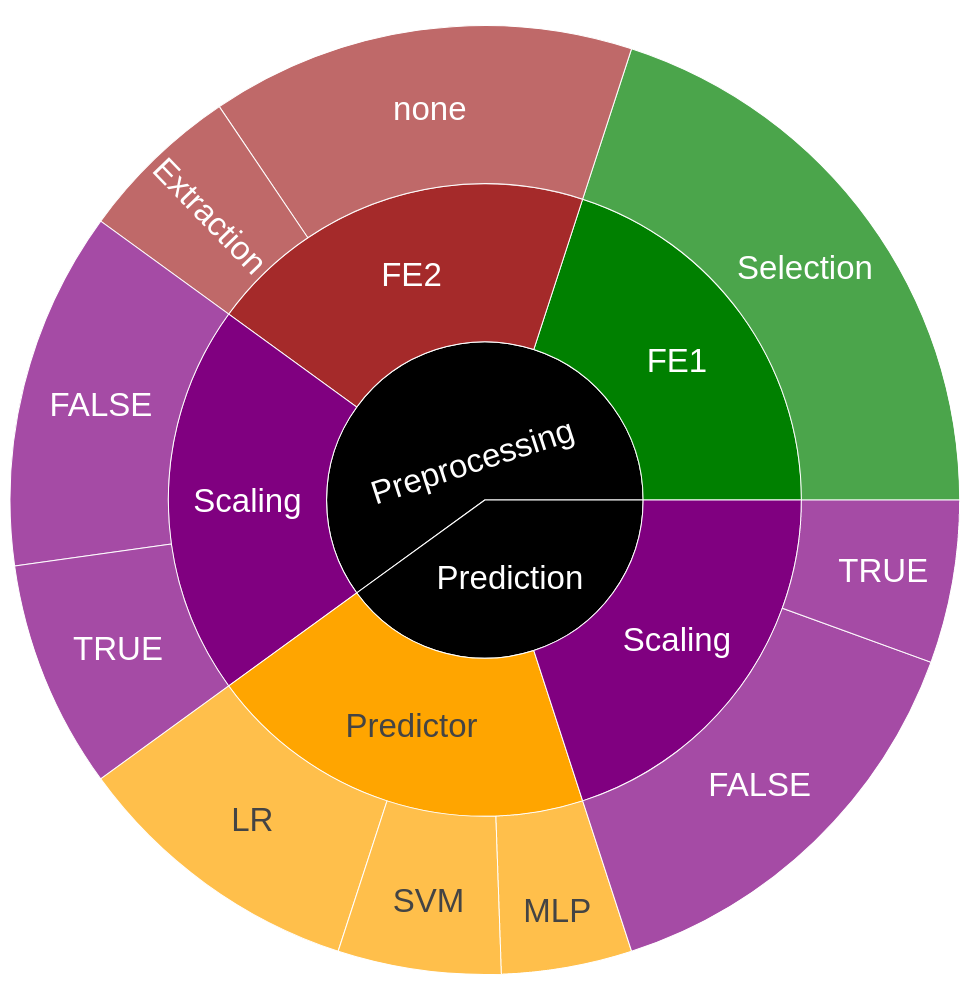
\includegraphics[width=5.5cm]{img/sunburst/ts.png}
    \caption{Pipeline composition for the different domains considered. From left to right: CV, NLP, and TS.}
    \label{fig:domain_composition}
    
    % [CV] prediction: LR (cifar10), SVM (fmnist), kNN (svhn)
    % [CV] preprocessing: increasingly used, in this order
    % 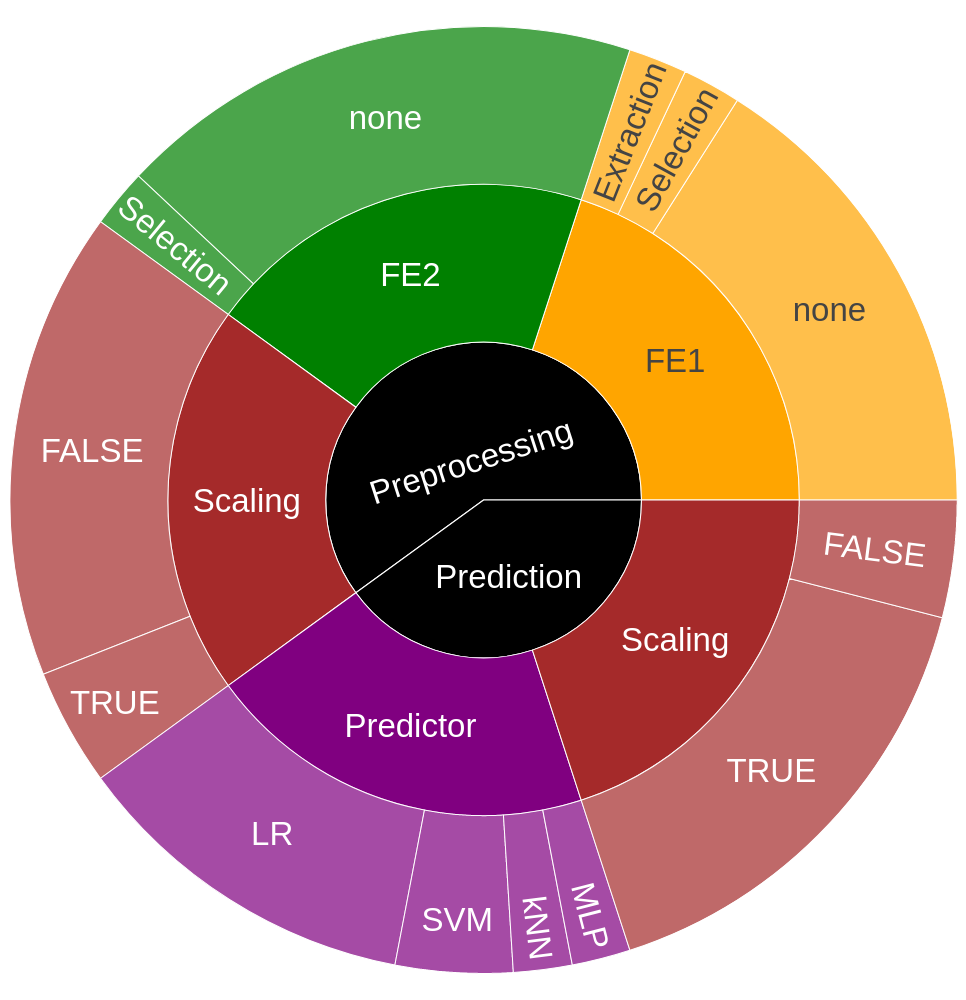
\includegraphics[width=5.5cm]{img/sunburst/cifar10.png}
    % 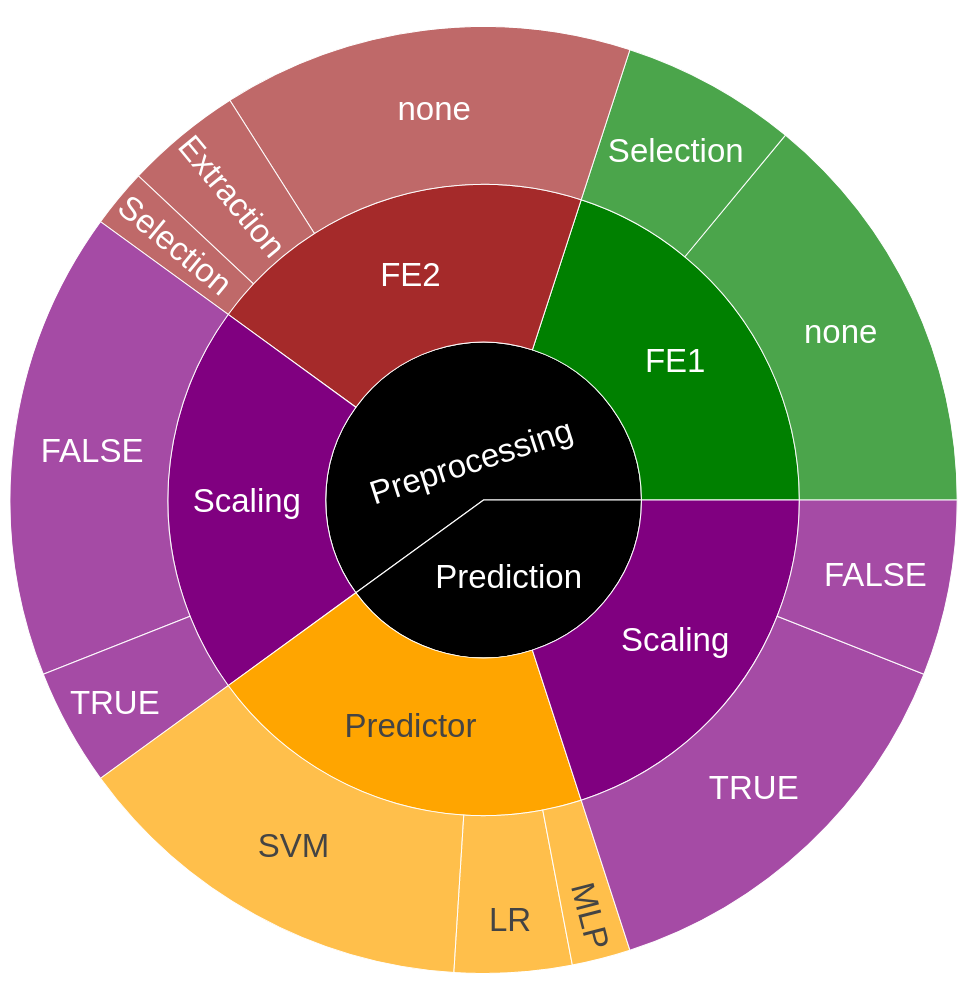
\includegraphics[width=5.5cm]{img/sunburst/fmnist.png}
    % 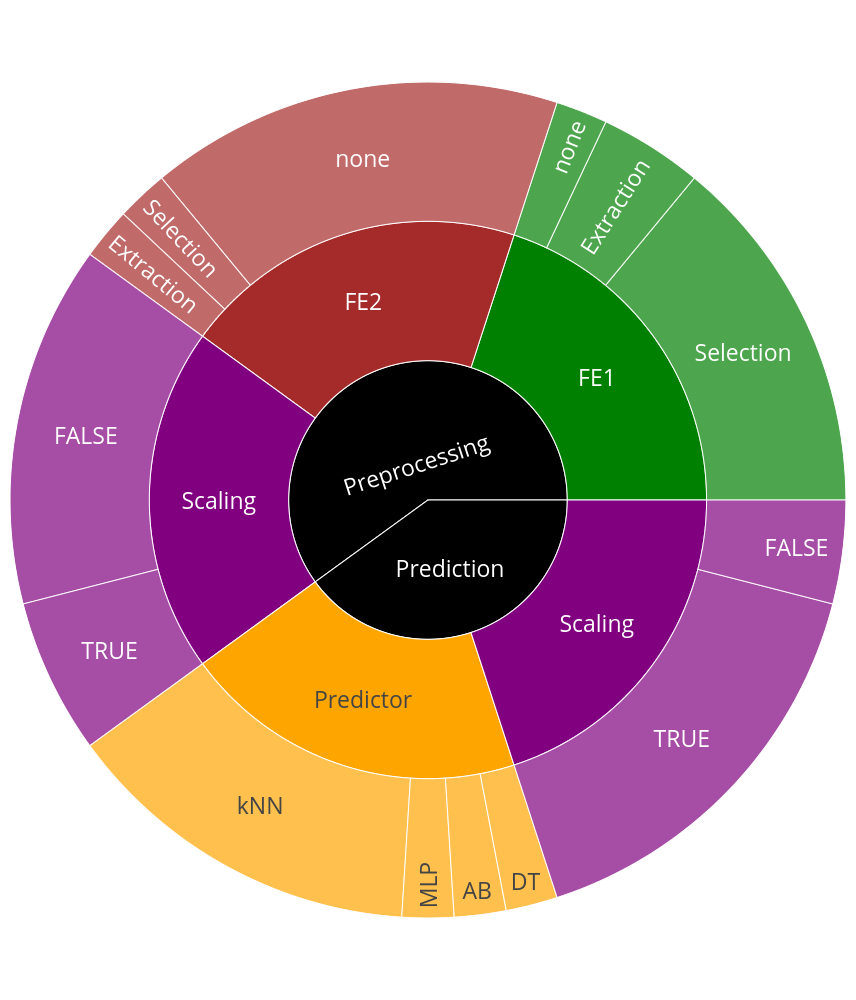
\includegraphics[width=5.5cm]{img/sunburst/svhn.png}
    
    % [TS] prediction: LR + SVM + MLP (natal), LR + SVM (boston)
    % 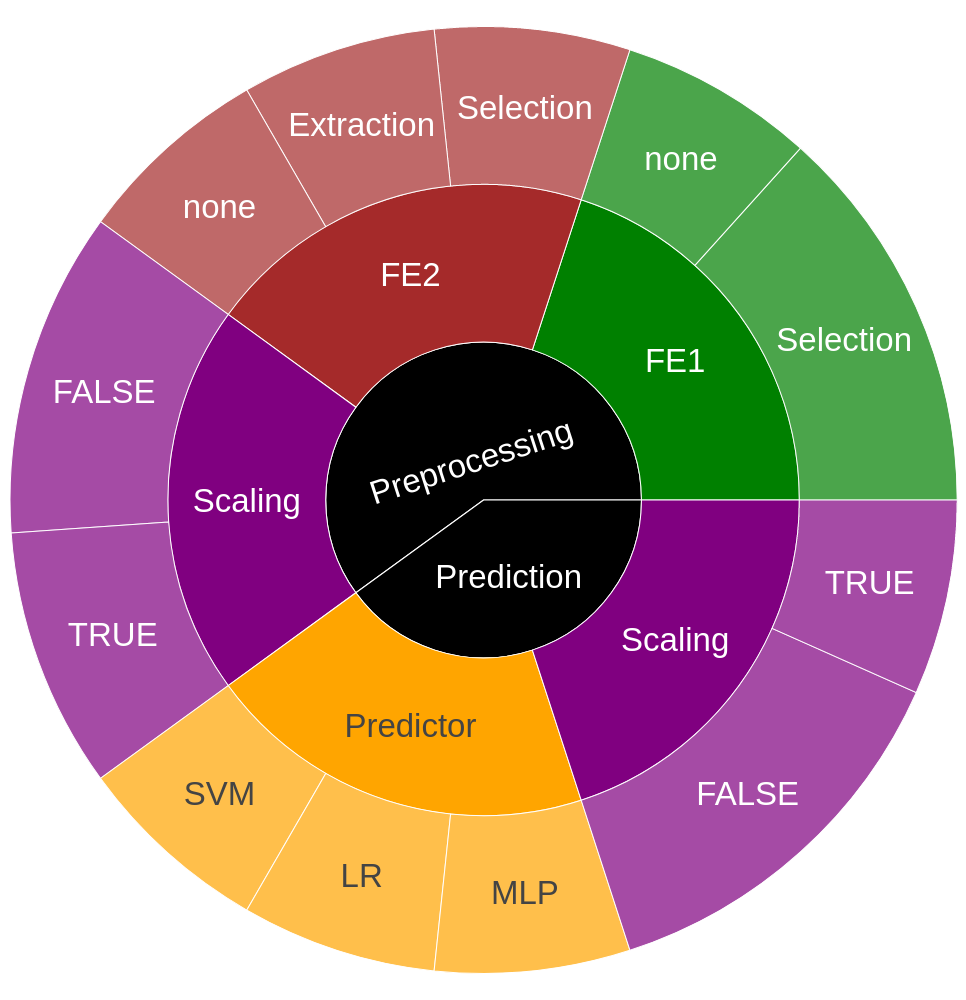
\includegraphics[width=5.5cm]{img/sunburst/natal.png}
    % 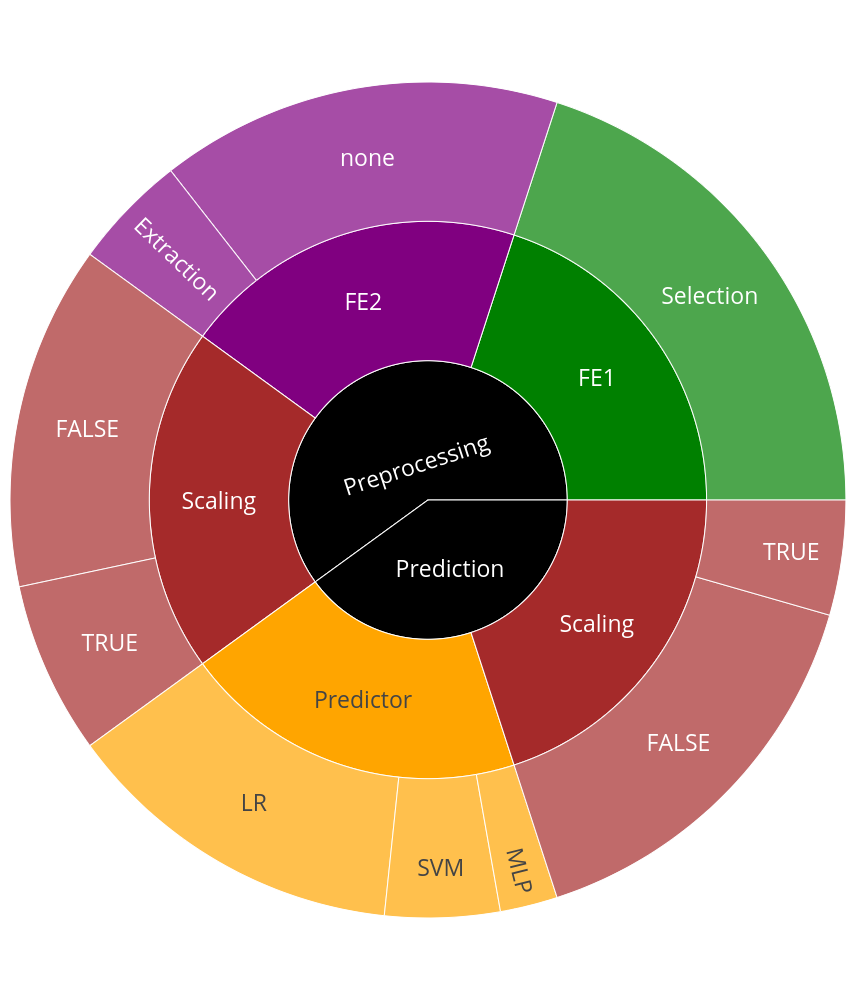
\includegraphics[width=5.5cm]{img/sunburst/boston.png}
    
    % [NLP] preprocessing: extraction -> selection (reuters)
    % 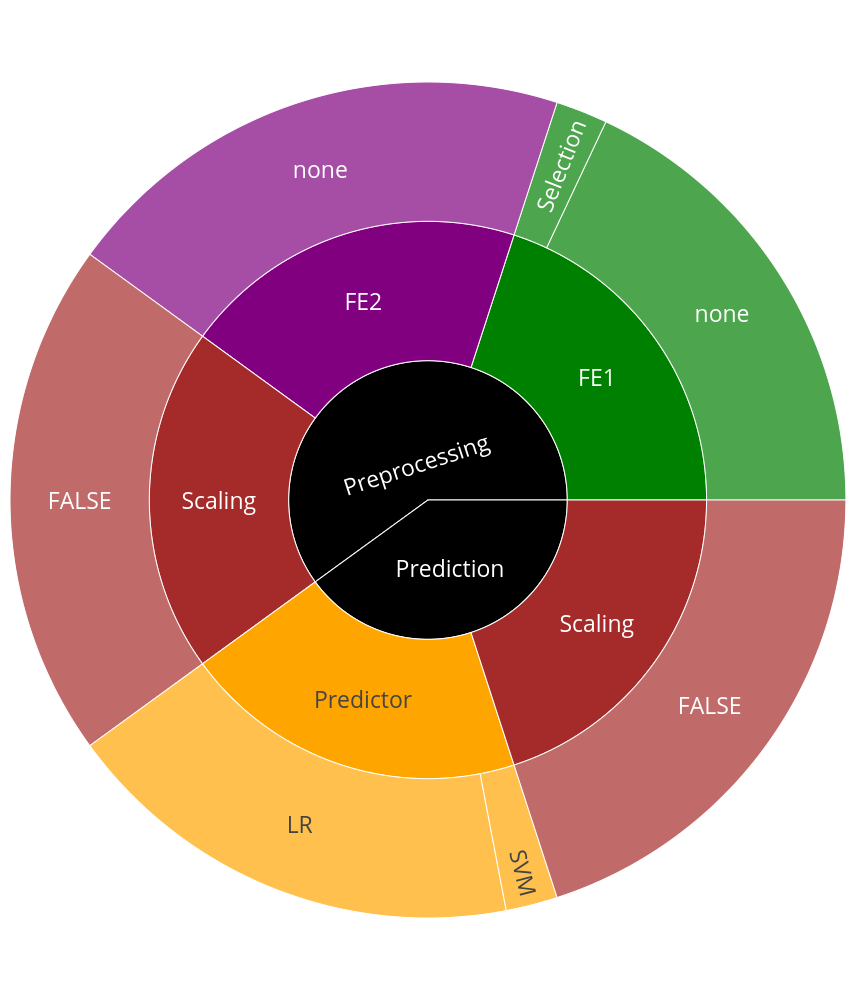
\includegraphics[width=5.5cm]{img/sunburst/lmrd.png}
    % 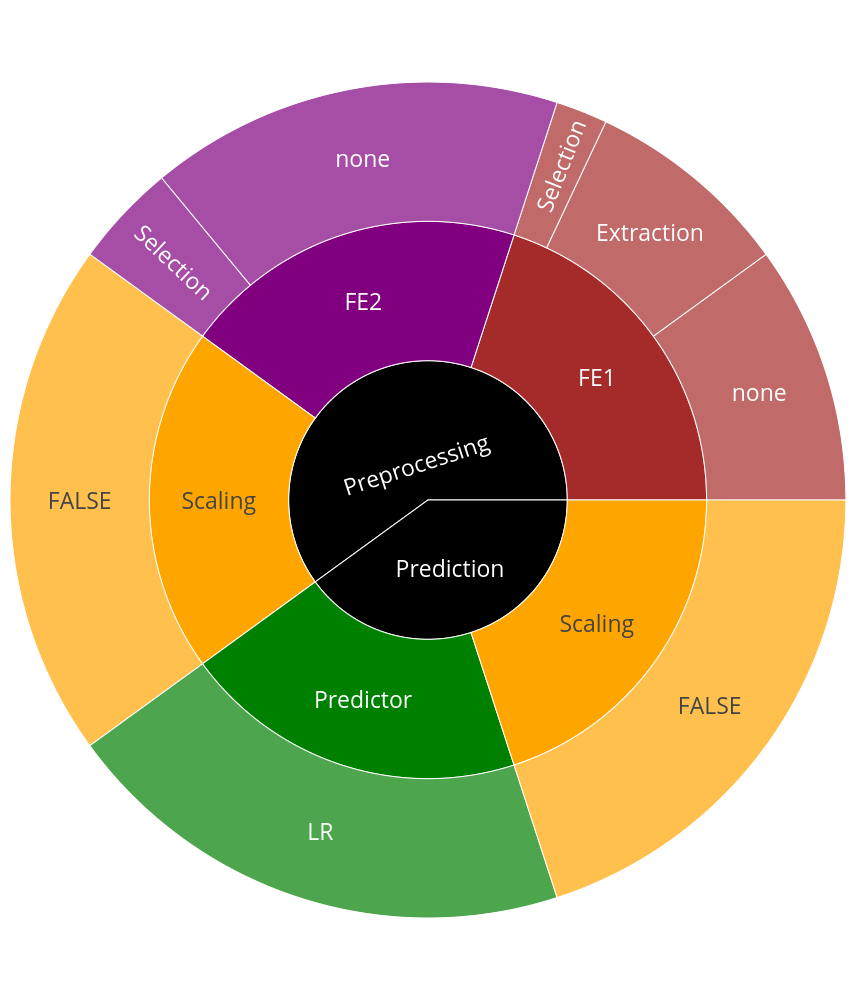
\includegraphics[width=5.5cm]{img/sunburst/reuters.png}
    % 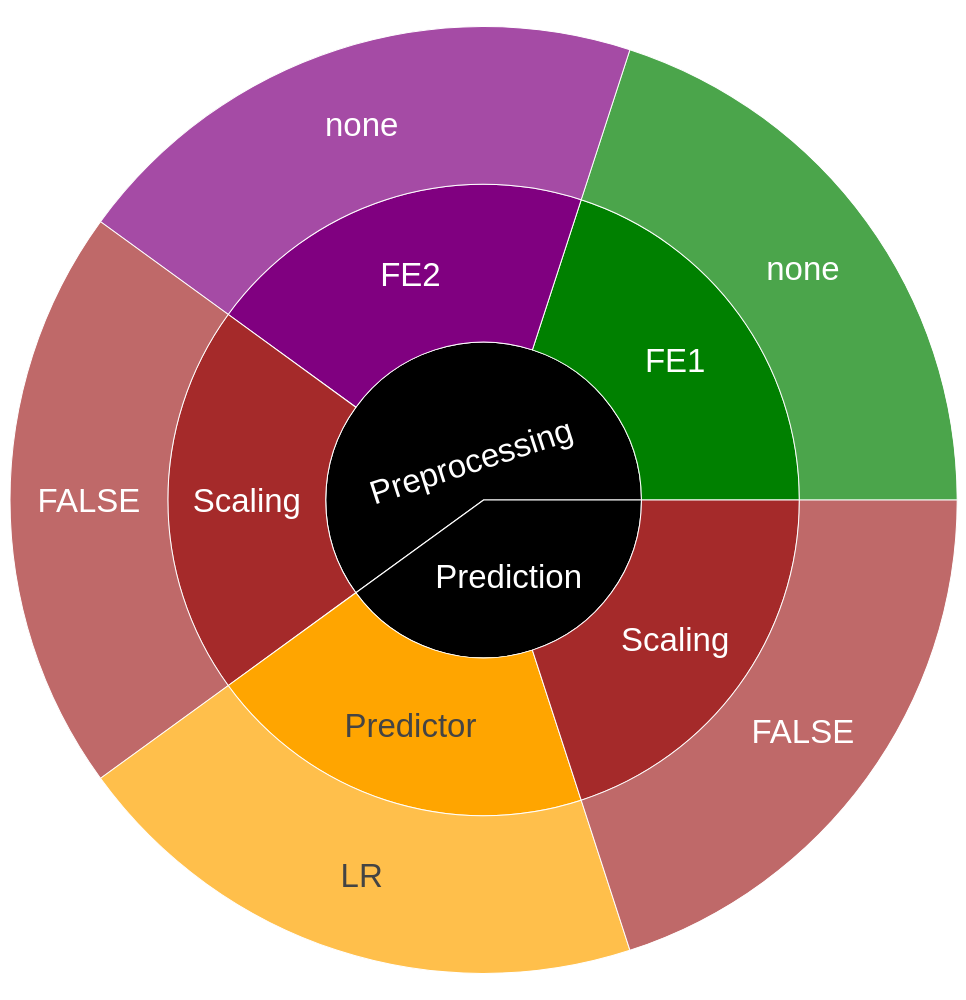
\includegraphics[width=5.5cm]{img/sunburst/agnews.png}
\end{figure*}

The compositions discussed above constitute strong evidence for the benefits of AutoML tools over manual selection and configuration. In addition, the simplicity of our template greatly improves the understanding of the pipelines selected. Finally, some of these observations might suggest the maximum runtime we fixed for each experiment for feasibility affects the composition of the pipelines. This possibility is further explored in Section~\ref{sec:alt-setups}. Nonetheless, the comparison of final scores for each dataset given in Table~\ref{tb:results} confirms that these pipelines are indeed high-performing w.r.t.~the provided configuration space and setup. Accuracy scores given for classification problems, as well as $R^2$ scores given for regression problems, are to be maximized. The best value per dataset is given in boldface. 

\begin{table*}[]
\centering
\caption{Accuracy~(\%) and $R^2$ scores (mean $\pm$ stand. deviation) for each dataset. The best algorithm per dataset is highlighted in boldface.}
\label{tb:results}
\scalebox{0.8}{\begin{tabular}{r|c|c|*{7}{c}|cc}
\hline  
\emph{Task} & \emph{Domain} & \emph{Dataset} & KNN & DT & RF & AB & MLP & SVM & LR & \isklearn & \textsc{AutoSklearn}\\ \hline
\multirow{6}{*}{\emph{Classification}} & \multirow{3}{*}{\emph{CV}} 
% & \emph{MNIST} & 96.88 & 87.76 & 94.16 & 72.99 & 95.82 & 11.35 & --- & \textbf{98.60} & 97.67\\ 
% \cline{3-12}
 & \emph{CIFAR-10} & 32.98 & 26.78$\pm0.27$ & 34.61$\pm0.35$ & 31.08 & 34.21$\pm0.37$ & 20.44 & 30.24 & 43.96$\pm6.95$ & \textbf{50.55}$\pm9.44$ \\ 
\cline{3-12}
%  & & \emph{CIFAR-100} & 15.04 & 08.48 & 13.39 & 07.03 & 01.00 & 04.50 & --- & \textbf{20.50} & \\ \cline{3-12}
 & & \emph{FMNIST} & 85.54 & 79.05$\pm0.17$ & 85.44$\pm0.14$ & 54.25 & 84.87$\pm0.52$ & 10.02 & 80.12 & \textbf{88.12}$\pm2.24$ & 79.88$\pm5.48$ \\ \cline{3-12}
 & & \emph{SVHN} & 46.83 & 42.17$\pm0.22$ & 56.51$\pm0.38$ & 22.78 & 19.58$\pm0.00$ & 0.00 & 23.94 & \textbf{58.02}$\pm15.52$ & 53.25$\pm10.41$ \\ \cline{2-12}
 & \multirow{3}{*}{\emph{NLP}} & \emph{LMRD} & 67.20 & 70.23$\pm0.15$ & 73.00$\pm0.64$ & 80.31 & 86.29$\pm0.09$ & 63.29 & 88.31 & \textbf{88.32}$\pm0.19$ & 88.01$\pm0.19$\\ \cline{3-12}
 &  & \emph{Reuters} & 77.74 & 70.41$\pm0.38$ & 69.32$\pm0.77$ & 47.55$\pm0.14$ & 80.59$\pm0.19$ & 36.20 & 79.07 & 81.57$\pm0.35$ & \textbf{82.57}$\pm1.01$ \\ 
 \cline{3-12}
 &  & \emph{AGNews} & 90.20 & 75.97$\pm0.22$ & 84.06$\pm0.41$ & 68.24 & 91.07$\pm0.19$ & 72.30 & 91.39 & \textbf{91.74}$\pm0.07$ & 91.57$\pm0.9$ \\ 
 \hline
\multirow{2}{*}{\emph{Regression}} & \multirow{2}{*}{\emph{TS}} & \emph{Natal} & 0.94 & 0.9134$\pm0.0022$ & 0.9538$\pm0.0047$ & 0.9185$\pm0.0089$ & 0.9547$\pm0.0016$ & 0.9389 & \textbf{0.9575} & 0.9538$\pm0.0022$ & 0.9549$\pm0.0087$\\
\cline{3-12}
 & & \emph{Boston} & 0.9576 & 0.9428$\pm0.0009$ & 0.9634$\pm0.0004$ & 0.9440$\pm0.0023$ & 0.9728$\pm0.0021$ & 0.8454 & 0.9743 & \textbf{0.9751}$\pm0.0001$ & 0.9707$\pm0.0006$\\
% \cline{2-12}
% & --- & \emph{NYC} & 0.6095 & 0.4477 & 0.6797 & 0.3821 & 0.5811 & 0.5495 & 0.4270 &  & 0.6991\\ 
\hline
\end{tabular}}
\end{table*}
As expected, pipelines devised by \isklearn and ensembles devised by \autosklearn present better performance than default models. The only exception is the Natal dataset, for which LR outperforms both AutoML tools. Comparing \isklearn and \autosklearn, it is remarkable that pipelines from the former are competitive with the ensembles from the latter. Indeed, the only datasets for which we see a non-negligible gap between the performance of the models devised by the two AutoML approaches are the three CV ones. For CIFAR-10, ensembles present higher mean, though at the cost of higher variance as well. For FMNIST and SVHN, it is the pipelines that achieve higher mean, though again at the cost of higher variance for the latter. Altogether, these results evidence the difficulty posed by computer vision problems when deep learning is not adopted. One likely explanation is the computational cost incurred by sample dimensionality, which becomes more critical in runtime-constrained scenarios. 
%Regarding Reuters, experiments reported on the supplementary material demonstrate that \irace initially converges to one or two predictors and then fine-tunes hyperparameters. In this case, \irace selected a well-performing predictor, based on the performance of the default models, but configuring MLPs is computationally costly, and likely would require more resources.

From a practical point of view, most of the pipelines engineered in this section could be deployed into a real-world production setup, due to their simplicity and performance. The only exceptions are CIFAR-10 and SVHN, for which both the pipelines from \isklearn and ensembles from \autosklearn still require improvements to produce estimators with a reasonable level of effectiveness.
%, which we investigate in the next section. 
In the next section, we investigate the effects of our proposed configuration space and setup in the performance of \isklearn.%, with a particular focus on CV. %Some of those experiments are also performed for NLP and TS, as we will discuss.
